\clearpage
\section*{Пятёрка 2. Вопросы 6–10}

% --- Вопрос 6 ---
\examquestion{6}{Метод Остроградского}
{Дайте обоснование методу выделения рациональной части интеграла от правильной рациональной дроби, знаменатель которой имеет кратные корни. Докажите корректность дифференцирования основного уравнения Остроградского для перехода к алгебраической системе линейных уравнений.}

\paragraph{Теоретическое обоснование метода.}
Пусть задан интеграл от правильной рациональной дроби $\int \frac{P(x)}{Q(x)} dx$, где многочлен знаменателя $Q(x)$ имеет кратные корни (действительные или комплексные), то есть его каноническое разложение имеет вид $Q(x) = (x-x_1)^{k_1}\dots(x^2+p_1x+q_1)^{m_1}\dots$. Традиционное разложение такой дроби на элементарные приводит к дробям высоких порядков, интегрирование которых требует применения громоздких рекуррентных формул понижения степени знаменателя.

Метод Остроградского позволяет обойти эту процедуру и чисто алгебраически выделить рациональную (алгебраическую) часть интеграла от трансцендентной части (логарифмы, арктангенсы). Основное уравнение метода имеет вид:
$$ \int \frac{P(x)}{Q(x)} dx = \frac{X(x)}{Q_1(x)} + \int \frac{Y(x)}{Q_2(x)} dx $$
где структура новых знаменателей однозначно определяется по исходному знаменателю $Q(x)$:
\begin{enumerate}
    \item $Q_1(x) = \text{НОД}(Q(x), Q'(x))$ — многочлен, содержащий все те же корни, что и $Q(x)$, но их кратности снижены ровно на единицу. Таким образом, $\frac{X(x)}{Q_1(x)}$ является искомой рациональной частью первообразной.
    \item $Q_2(x) = \frac{Q(x)}{Q_1(x)}$ — многочлен, содержащий все корни знаменателя $Q(x)$, но строго первой кратности. Дробь $\frac{Y(x)}{Q_2(x)}$ под интегралом даст исключительно трансцендентные функции.
\end{enumerate}
Степени неопределенных многочленов числителей выбираются на единицу меньше степеней соответствующих знаменателей: $\deg X = \deg Q_1 - 1$, $\deg Y = \deg Q_2 - 1$.

\paragraph{Доказательство корректности дифференцирования.}
Для нахождения коэффициентов многочленов $X(x)$ и $Y(x)$ выполним операцию дифференцирования обеих частей основного уравнения по переменной $x$. На основании основной теоремы дифференциального исчисления, производная от неопределенного интеграла по его верхнему пределу равна подынтегральной функции:
$$ \frac{P(x)}{Q(x)} = \frac{X'(x)Q_1(x) - X(x)Q_1'(x)}{Q_1^2(x)} + \frac{Y(x)}{Q_2(x)} $$
Докажем, что полученное уравнение легко сводится к линейной системе уравнений. Умножим обе части равенства на исходный многочлен $Q(x)$. Учитывая, что по определению $Q(x) = Q_1(x)Q_2(x)$, получаем:
$$ P(x) = \frac{\big(X'(x)Q_1(x) - X(x)Q_1'(x)\big) \cdot Q_1(x)Q_2(x)}{Q_1^2(x)} + \frac{Y(x) \cdot Q_1(x)Q_2(x)}{Q_2(x)} $$
Сокращая дроби, приходим к уравнению:
$$ P(x) = \frac{X'(x)Q_1(x)Q_2(x) - X(x)Q_1'(x)Q_2(x)}{Q_1(x)} + Y(x)Q_1(x) $$
Поскольку $Q_2(x) = \frac{Q(x)}{Q_1(x)}$, то выражение $\frac{Q_1'(x)Q_2(x)}{Q_1(x)}$ является целым многочленом. Действительно, $Q'(x) = (Q_1(x)Q_2(x))' = Q_1'(x)Q_2(x) + Q_1(x)Q_2'(x)$. Разделив на $Q_1(x)$, видим, что все слагаемые целочисленны по структуре степеней. Окончательно получаем алгебраическое тождество многочленов:
$$ P(x) = X'(x)Q_2(x) - X(x) \, \frac{Q_1'(x)Q_2(x) - Q'(x)}{Q_1(x)} + Y(x)Q_1(x) $$
Левая и правая части полученного тождества представляют собой многочлены. Приравнивая коэффициенты при одинаковых степенях $x$, мы получаем совместную систему линейных алгебраических уравнений. Корректность гарантируется линейной независимостью базисных дробей разложения.

\paragraph{Бонус-пример:} Применим метод к интегралу $\int \frac{dx}{(x^2-1)^2}$. Здесь $Q(x) = (x^2-1)^2$.
\begin{itemize}
    \item Находим знаменатели: $Q'(x) = 2(x^2-1)\cdot 2x = 4x(x^2-1)$. Тогда $Q_1(x) = \text{НОД}(Q, Q') = x^2-1$. Соответственно, $Q_2(x) = \frac{Q(x)}{Q_1(x)} = x^2-1$.
    \item Записываем структуру числителей: так как $\deg Q_1 = 2$ и $\deg Q_2 = 2$, то $\deg X = 1 \implies X(x) = Ax + B$, $\deg Y = 1 \implies Y(x) = Cx + D$.
    \item Формула Остроградского: $\int \frac{dx}{(x^2-1)^2} = \frac{Ax+B}{x^2-1} + \int \frac{Cx+D}{x^2-1} dx$. Дифференцируем:
    $$ \frac{1}{(x^2-1)^2} = \frac{A(x^2-1) - 2x(Ax+B)}{(x^2-1)^2} + \frac{Cx+D}{x^2-1} \implies 1 = A(x^2-1) - 2x(Ax+B) + (Cx+D)(x^2-1) $$
    Раскрывая скобки и приравнивая коэффициенты, находим: $A = 0, B = -1/2, C = 0, D = -1/2$.
    \item Итог: $\int \frac{dx}{(x^2-1)^2} = -\frac{x}{2(x^2-1)} - \frac{1}{4}\ln\left|\frac{x-1}{x+1}\right| + C$.
\end{itemize}

% --- Вопрос 7 ---
\examquestion{7}{Интегрирование дробно-линейных иррациональностей}
{Опираясь на понятие рационализирующей подстановки, подробно разберите метод интегрирования выражений, содержащих дробно-линейные иррациональности вида $\sqrt[n]{\frac{ax+b}{cx+d}}$. Докажите теорему о сведении таких интегралов к интегралам от рациональных функций.}

\begin{theorem}[О рационализации дробно-линейных иррациональностей]
Интеграл вида $\int R\left(x, \sqrt[n]{\frac{ax+b}{cx+d}}\right) dx$, где $R$ — рациональная функция своих аргументов, а $ad - bc \neq 0$, с помощью подстановки $t = \sqrt[n]{\frac{ax+b}{cx+d}}$ всегда сводится к интегралу от рациональной функции переменной $t$.
\end{theorem}

\begin{proof}
Пусть $t = \sqrt[n]{\frac{ax+b}{cx+d}}$. Для доказательства теоремы необходимо показать, что переменная $x$ и её дифференциал $dx$ выражаются через целые рациональные степени переменной $t$. Возведем обе части равенства в степень $n$:
$$ t^n = \frac{ax+b}{cx+d} $$
Выразим отсюда $x$. Для этого умножим обе части на знаменатель $cx+d$:
$$ t^n(cx + d) = ax + b \implies c x t^n + d t^n = a x + b \implies x(c t^n - a) = b - d t^n $$
Отсюда получаем явное выражение для переменной $x$ как рациональной функции от $t$:
$$ x = \frac{b - d t^n}{c t^n - a} = \psi(t) $$
Поскольку функция $\psi(t)$ является дробно-рациональной (отношение двух многочленов), её производная по переменной $t$ также будет являться дробно-рациональной функцией. Найдем дифференциал $dx$:
$$ dx = \psi'(t)dt = \frac{(-d \cdot n t^{n-1})(c t^n - a) - (b - d t^n)(c \cdot n t^{n-1})}{(c t^n - a)^2} dt = \frac{n t^{n-1}(ad - bc)}{(c t^n - a)^2} dt $$
Подставим полученные выражения в исходный интеграл:
$$ \int R\left(x, \sqrt[n]{\frac{ax+b}{cx+d}}\right) dx = \int R\left( \psi(t), t \right) \psi'(t) dt $$
Так как суперпозиция и произведение рациональных функций представляют собой рациональную функцию, подынтегральное выражение становится чистой рациональной дробью от переменной $t$. Теорема доказана.
\end{proof}

\paragraph{Бонус-пример:} Вычислим интеграл $\int \frac{dx}{(1+x)\sqrt{x}}$.
Данный интеграл содержит простую линейную иррациональность $\sqrt{x}$. Сделаем замену $t = \sqrt{x} \implies x = t^2$, следовательно, $dx = 2t\,dt$. Подставляем выражения в исходный интеграл:
$$ \int \frac{2t\,dt}{(1+t^2) \cdot t} = 2 \int \frac{dt}{1+t^2} = 2 \arctan t + C $$
Выполняя обратную замену $t = \sqrt{x}$, получаем окончательный ответ: $2 \arctan\sqrt{x} + C$.

% --- Вопрос 8 ---
\examquestion{8}{Подстановки Эйлера}
{Сформулируйте геометрические и алгебраические предпосылки трех подстановок Эйлера для интегралов вида $\int R(x, \sqrt{ax^2+bx+c})dx$. Выведите формулы для первой и второй подстановок Эйлера, доказав их рационализирующий характер.}

\paragraph{Алгебраические предпосылки.}
Интегралы вида $\int R(x, \sqrt{ax^2+bx+c})dx$ не могут быть вычислены в элементарных функциях напрямую, если квадратный трехчлен не является полным квадратом. Эйлер предложил три подстановки, основанные на алгебраической структуре коэффициентов трехчлена, которые переводят кривую второго порядка в параметрический вид, выражаемый рациональными функциями.

\paragraph{Вывод первой подстановки Эйлера ($a > 0$).}
Если старший коэффициент квадратного трехчлена положителен, то при очень больших $x$ поведение корня близко к поведению функции $\pm \sqrt{a}x$. Это позволяет сделать замену:
$$ \sqrt{ax^2+bx+c} = \pm\sqrt{a}x + t $$
Выберем знак «+» и возведем обе части равенства в квадрат для уничтожения радикалов:
$$ ax^2 + bx + c = (\sqrt{a}x + t)^2 = ax^2 + 2\sqrt{a}xt + t^2 $$
Слагаемые $ax^2$ в левой и правой частях взаимно уничтожаются, что линеаризует уравнение относительно $x$:
$$ bx + c = 2\sqrt{a}xt + t^2 \implies x(b - 2\sqrt{a}t) = t^2 - c $$
Отсюда получаем строго рациональное выражение переменной $x$ через параметр $t$:
$$ x = \frac{t^2 - c}{b - 2\sqrt{a}t} $$
Соответственно, дифференциал $dx = \left(\frac{t^2 - c}{b - 2\sqrt{a}t}\right)' dt$ и сам радикал также становятся рациональными функциями от $t$, что доказывает рационализирующий характер подстановки.

\paragraph{Вывод второй подстановки Эйлера ($c > 0$).}
Если свободный член положителен, то при $x=0$ значение радикала равно $\pm\sqrt{c}$. Это позволяет связать радикал с переменной $x$ через новый параметр $t$:
$$ \sqrt{ax^2+bx+c} = xt \pm \sqrt{c} $$
Выберем знак «+» и возведем равенство в квадрат:
$$ ax^2 + bx + c = (xt + \sqrt{c})^2 = x^2t^2 + 2\sqrt{c}xt + c $$
Уничтожая константу $c$ в обеих частях, получаем уравнение:
$$ ax^2 + bx = x^2t^2 + 2\sqrt{c}xt $$
Разделим обе части на $x$ (предполагая $x \neq 0$), что снова линеаризует уравнение по переменной $x$:
$$ ax + b = xt^2 + 2\sqrt{c}t \implies x(a - t^2) = 2\sqrt{c}t - b $$
Получаем рациональное выражение для $x$:
$$ x = \frac{2\sqrt{c}t - b}{a - t^2} $$
Дифференциал $dx$ и корень выражаются через рациональные дроби от $t$, интеграл успешно рационализируется.

\paragraph{Бонус-пример (Первая подстановка Эйлера):}
Вычислим $\int \frac{dx}{\sqrt{x^2+1}}$. Здесь $a=1>0, c=1$. Применяем первую подстановку Эйлера: $\sqrt{x^2+1} = -x + t \implies x^2+1 = x^2 - 2xt + t^2 \implies 1 = -2xt + t^2 \implies x = \frac{t^2-1}{2t}$.
Дифференциал: $dx = \frac{1}{2}\left(1 + \frac{1}{t^2}\right)dt = \frac{t^2+1}{2t^2}dt$. Выразим радикал: $\sqrt{x^2+1} = t - \frac{t^2-1}{2t} = \frac{t^2+1}{2t}$. Подставляем в интеграл:
$$ \int \frac{\frac{t^2+1}{2t^2}dt}{\frac{t^2+1}{2t}} = \int \frac{dt}{t} = \ln|t| + C = \ln\left|x + \sqrt{x^2+1}\right| + C. $$

% --- Вопрос 9 ---
\examquestion{9}{Дифференциальный бином Чебышёва}
{Сформулируйте теорему Чебышёва об интегрировании дифференциального бинома. Проведите подробный разбор трех условий Чебышёва с указанием замен, переводящих интеграл вида $\int x^{m}(a+bx^{n})^{p}dx$ к интегралу от рациональной функции.}

\begin{theorem}[Теорема Чебышёва]
Интеграл от дифференциального бинома $\int x^{m}(a+bx^{n})^{p}dx$, где $m, n, p$ — рациональные числа, а $a, b \in \mathbb{R} \setminus \{0\}$, выражается в элементарных функциях (интегрируется в конечном виде) тогда и только тогда, когда выполняется одно из следующих трех условий Чебышёва. Во всех остальных случаях интеграл является «неберущимся» в элементарных функциях.
\end{theorem}

\paragraph{Подробный разбор трех условий и замен:}
Прежде чем применять условия, выполняется базовая замена переменной для упрощения структуры степеней: $z = x^n \implies x = z^{1/n} \implies dx = \frac{1}{n}z^{\frac{1}{n}-1}dz$. Интеграл принимает вид $\frac{1}{n}\int z^{\frac{m+1}{n}-1}(a+bz)^p dz$. Это приводит к исследованию следующих случаев:

\begin{enumerate}
    \item \textbf{Первое условие: $p$ — целое число ($p \in \mathbb{Z}$).}
    \\ Если показатель степени $p$ является целым числом, то подынтегральное выражение представляет собой сумму дробно-рациональных степеней независимой переменной $x$. 
    \\ \textit{Рационализирующая подстановка:} Пусть $\lambda$ — наименьшее общее кратное (НОК) знаменателей рациональных дробей $m$ и $n$. Тогда замена $x = t^\lambda$ полностью уничтожает дробные степени аргумента $x$, приводя выражение к многочлену или правильной рациональной дроби.
    
    \item \textbf{Второе условие: $\frac{m+1}{n}$ — целое число ($\frac{m+1}{n} \in \mathbb{Z}$).}
    \\ В этом случае после базовой замены переменная $z$ вне скобок оказывается в целой степени, а дробной остается только степень выражения под скобкой.
    \\ \textit{Рационализирующая подстановка:} Пусть $s$ — знаменатель рационального числа $p$ ($p = r/s$). Тогда применяется замена:
    $$ a + bx^n = t^s $$
    Отсюда выражается $x^n = \frac{t^s - a}{b}$, что позволяет получить строго рациональные выражения для всех компонентов подынтегральной функции.
    
    \item \textbf{Третье условие: $\frac{m+1}{n} + p$ — целое число ($\frac{m+1}{n} + p \in \mathbb{Z}$).}
    \\ В данном случае ни $p$, ни $\frac{m+1}{n}$ по отдельности не являются целыми числами, но их сумма дает целое число. Для извлечения выгоды из этого скрытого тождества бином искусственно преобразуется путем вынесения $x^n$ за скобки: $x^m(a+bx^n)^p = x^m \cdot (x^n)^p \cdot (ax^{-n} + b)^p = x^{m+np}(ax^{-n}+b)^p$.
    \\ \textit{Рационализирующая подстановка:} Пусть $s$ — знаменатель рационального числа $p$. Замена имеет вид:
    $$ a x^{-n} + b = t^s \quad \text{или} \quad \frac{a+bx^n}{x^n} = t^s $$
    Дифференцирование данного выражения приводит к полному взаимному сокращению иррациональностей.
\end{enumerate}

\paragraph{Бонус-пример (Второе условие Чебышёва):}
Вычислим интеграл $\int \frac{\sqrt{1+\sqrt[3]{x}}}{x} dx = \int x^{-1}(1+x^{1/3})^{1/2} dx$.
Здесь $m = -1, n = 1/3, p = 1/2$. Проверим второе условие: $\frac{m+1}{n} = \frac{-1+1}{1/3} = 0 \in \mathbb{Z}$. Условие выполнено. Знаменатель $p$ равен $s=2$.
Применяем подстановку: $1 + x^{1/3} = t^2 \implies x^{1/3} = t^2 - 1 \implies x = (t^2-1)^3$. Находим дифференциал: $dx = 3(t^2-1)^2 \cdot 2t \, dt = 6t(t^2-1)^2 dt$. Подставляем:
$$ \int \frac{t}{(t^2-1)^3} \cdot 6t(t^2-1)^2 dt = 6 \int \frac{t^2}{t^2-1} dt = 6 \int \left(1 + \frac{1}{t^2-1}\right) dt = 6t + 3\ln\left|\frac{t-1}{t+1}\right| + C $$
где $t = \sqrt{1+\sqrt[3]{x}}$.

% --- Вопрос 10 ---
\examquestion{10}{Определенный интеграл Римана}
{Сформулируйте понятие определенного интеграла Римана через конструкции разбиения, размеченного разбиения и интегральных сумм. Докажите теорему о необходимом условии интегрируемости функции по Риману (ограниченность функции).}

\paragraph{Конструкции интеграла Римана.}
Пусть функция $f(x)$ задана на конечном отрезке $[a, b]$ ($a < b$). 
\begin{enumerate}
    \item \textbf{Разбиение отрезка:} Назовем разбиением $T$ отрезка $[a, b]$ конечный упорядоченный набор точек $a = x_0 < x_1 < \dots < x_{n-1} < x_n = b$. Эти точки делят отрезок на $n$ элементарных отрезков $[x_{k-1}, x_k]$ длины $\Delta x_k = x_k - x_{k-1}$.
    \\ Параметром (или мелкостью) разбиения $T$ называется длина наибольшего элементарного отрезка: $\delta(T) = \max_{1 \le k \le n} \Delta x_k$.
    
    \item \textbf{Размеченное разбиение:} Если на каждом элементарном отрезке $[x_{k-1}, x_k]$ выбрана точка $\xi_k \in [x_{k-1}, x_k]$, то совокупность точек $\xi = \{\xi_1, \dots, \xi_n\}$ называется разметкой разбиения $T$, а пара $(T, \xi)$ — размеченным разбиением.
    
    \item Векторное графическое представление разбиения отрезка и построения ступенчатых прямоугольников интегральной суммы Римана:
    \begin{center}
    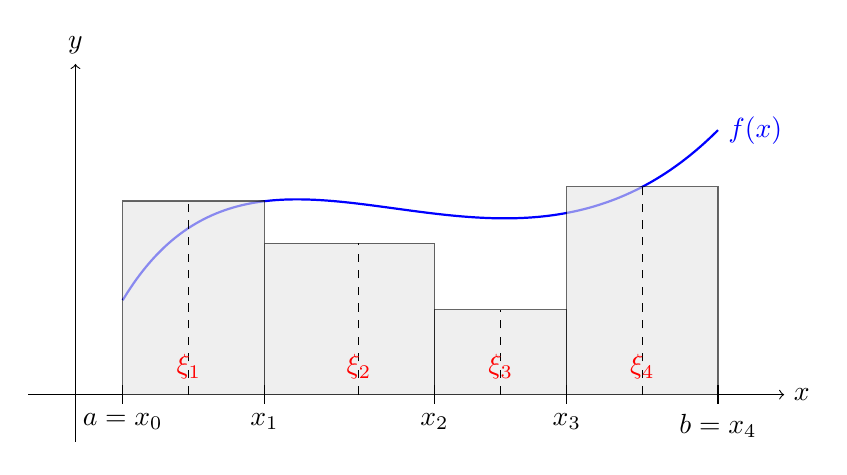
\begin{tikzpicture}[scale=1.2]
        \draw[->] (-0.5,0) -- (7.5,0) node[right] {$x$};
        \draw[->] (0,-0.5) -- (0,3.5) node[above] {$y$};
        
        % Функция
        \draw[thick, blue] (0.5,1) .. controls (2.0,3.5) and (4.5,0.5) .. (6.8,2.8) node[right] {$f(x)$};
        
        % Отрезок 1
        \draw[fill=gray!20, opacity=0.6] (0.5,0) rectangle (2.0, 2.05);
        \draw[dashed] (1.2,0) -- (1.2, 2.05);
        \node[above=2pt, red] at (1.2,0) {$\xi_1$};
        
        % Отрезок 2
        \draw[fill=gray!20, opacity=0.6] (2.0,0) rectangle (3.8, 1.6);
        \draw[dashed] (3.0,0) -- (3.0, 1.6);
        \node[above=2pt, red] at (3.0,0) {$\xi_2$};
        
        % Отрезок 3
        \draw[fill=gray!20, opacity=0.6] (3.8,0) rectangle (5.2, 0.9);
        \draw[dashed] (4.5,0) -- (4.5, 0.9);
        \node[above=2pt, red] at (4.5,0) {$\xi_3$};
        
        % Отрезок 4
        \draw[fill=gray!20, opacity=0.6] (5.2,0) rectangle (6.8, 2.2);
        \draw[dashed] (6.0,0) -- (6.0, 2.2);
        \node[above=2pt, red] at (6.0,0) {$\xi_4$};
        
        % Точки разбиения x_i (под осью)
        \draw (0.5, 0.1) -- (0.5, -0.1) node[below] {$a=x_0$};
        \draw (2.0, 0.1) -- (2.0, -0.1) node[below] {$x_1$};
        \draw (3.8, 0.1) -- (3.8, -0.1) node[below] {$x_2$};
        \draw (5.2, 0.1) -- (5.2, -0.1) node[below] {$x_3$};
        \draw (6.8, 0.1) -- (6.8, -0.1) node[below] {$b=x_4$};
    \end{tikzpicture}
    \end{center}
    
    \item \textbf{Интегральная сумма Римана:} Для функции $f(x)$ и размеченного разбиения $(T, \xi)$ интегральная сумма имеет вид:
    $$ \sigma(f, T, \xi) = \sum_{k=1}^n f(\xi_k) \Delta x_k $$
    
    \item \textbf{Определение интеграла Римана:} Число $I$ называется пределом интегральных сумм Римана при мелкости разбиения $\delta(T) \to 0$, если $\forall \varepsilon > 0$ существует $\exists \space \delta_0 > 0$ такое, что для любого разбиения $T$ с параметром $\delta(T) < \delta_0$ и при любом выборе точек разметки $\xi$ выполняется неравенство:
    $$ |\sigma(f, T, \xi) - I| < \varepsilon $$
    В этом случае функция $f(x)$ называется интегрируемой по Риману на отрезке $[a, b]$, а число $I$ обозначается как $\int_a^b f(x) dx$.
\end{enumerate}

\begin{theorem}[Необходимое условие интегрируемости Римана]
Если функция $f(x)$ интегрируема по Риману на отрезке $[a, b]$, то она ограничена на этом отрезке.
\end{theorem}

\begin{proof}
Докажем от противного. Пусть функция $f(x)$ интегрируема на $[a, b]$, то есть существует конечный предел интегральных сумм $\lim_{\delta(T) \to 0} \sigma(f, T, \xi) = I$, но при этом $f(x)$ является неограниченной на $[a, b]$.

Зафиксируем значение $\varepsilon = 1$. Из определения интегрируемости следует, что существует такое число $\delta_0 > 0$, что для любого разбиения $T$ с мелкостью $\delta(T) < \delta_0$ и для любой разметки $\xi$ выполняется неравенство:
$$ |\sigma(f, T, \xi) - I| < 1 \implies |\sigma(f, T, \xi)| < |I| + 1 $$
Зафиксируем какое-нибудь одно разбиение $T$, удовлетворяющее условию $\delta(T) < \delta_0$. Так как функция $f(x)$ неограничена на всем отрезке $[a, b]$, она обязана быть неограниченной хотя бы на одном из элементарных отрезков нашего разбиения. Пусть этот отрезок имеет номер $k$, то есть функция неограничена на $[x_{k-1}, x_k]$.

Разобьем интегральную сумму на два слагаемых, выделив отдельно $k$-й элемент:
$$ \sigma(f, T, \xi) = f(\xi_k)\Delta x_k + \sum_{i \neq k} f(\xi_i)\Delta x_i $$
Обозначим фиксированную сумму по всем остальным отрезкам за константу $C = \sum_{i \neq k} f(\xi_i)\Delta x_i$. Она полностью неизменна, если мы зафиксируем точки разметки $\xi_i$ во всех промежутках, кроме $k$-го. Тогда $\sigma(f, T, \xi) = f(\xi_k)\Delta x_k + C$.

Так как функция $f(x)$ неограничена на отрезке $[x_{k-1}, x_k]$, мы можем выбрать точку разметки $\xi_k$ таким образом, чтобы значение $|f(\xi_k)|$ оказалось сколь угодно большим. Выберем точку $\xi_k$ так, чтобы выполнялось строгое неравенство:
$$ |f(\xi_k)| > \frac{|I| + 1 + |C|}{\Delta x_k} $$
Умножим обе части на длину отрезка $\Delta x_k > 0$:
$$ |f(\xi_k)\Delta x_k| > |I| + 1 + |C| $$
Используя алгебраическое неравенство треугольника в форме $|A + B| \ge |A| - |B|$, оценим модуль полной интегральной суммы:
$$ |\sigma(f, T, \xi)| = |f(\xi_k)\Delta x_k + C| \ge |f(\xi_k)\Delta x_k| - |C| $$
Подставляя нашу нижнюю оценку для $|f(\xi_k)\Delta x_k|$, получаем:
$$ |\sigma(f, T, \xi)| > \big(|I| + 1 + |C|\big) - |C| = |I| + 1 $$
Таким образом, мы нашли такую разметку, для которой $|\sigma(f, T, \xi)| > |I| + 1$. Однако это прямо противоречит неравенству, полученному из предположения об интегрируемости функции. Полученное противоречие доказывает, что функция обязана быть ограниченной.
\end{proof}

\paragraph{Бонус-пример (Функция Дирихле):}
Рассмотрим классический пример ограниченной, но не интегрируемой по Риману функции — функцию Дирихле $\chi(x)$ на отрезке $[0, 1]$, которая равна $1$, если $x$ рационально, и $0$, если $x$ иррационально. 
\\ Функция строго ограничена ($0 \le \chi(x) \le 1$). Однако для любого разбиения $T$, если мы выберем разметку $\xi$ состоящей только из рациональных чисел, интегральная сумма будет равна: $\sum 1 \cdot \Delta x_k = 1$. Если же выбрать точки разметки из иррациональных чисел, то сумма равна $\sum 0 \cdot \Delta x_k = 0$. Предел интегральных сумм не существует, так как значение зависит от выбора разметки при любой мелкости разбиения. Функция не интегрируема по Риману.